As human beings, we have always relied on certain social constructs to guide our interactions and transactions with one another. Money and trust are two such constructs that have played a vital role in shaping our societies, and the way we live our lives. However, the digital age has brought with it new challenges that are testing the foundations of these social norms.\par
In a world where we are increasingly connected through the internet and able to communicate with people from all corners of the globe, the concept of money and trust is changing. Gone are the days of the village structure in which we evolved, where personal relationships and face-to-face interactions were ubiquitous. Now, we are faced with the prospect of working and interacting one another, and also with artificial intelligence actors that seem subjectively real, all while navigating the complexities of a global mixed reality.\par
This transition to a more efficient and interconnected world has the potential to bring about great benefits, but it also presents us with an enormous challenge. The chaotic and intangible mix of value, trust, socialisation, generative art, and AI chat actors, is not yet well understood, and it will take time for us to adapt to this new way of living and interacting with one another.\par
We initially wanted to explore exciting new developments in the transmission of value, and trust, in `digital society'. The problem is that each of these topics alone are enormously complex, and the intersections seem to be more so. We have been researching the current state-of-the-art, and the emerging consensus narrative, to try to figure out how the collision of these technologies might serve our virtual production workflows (Figure \ref{fig:pathway}). As we worked on this research the Cambrian explosion of generative AI added an incredibly important new strand to our investigation.\par
Over the course of a couple of years the focus of the work has developed, and refined. Our tool-kit, as it stands, supports inclusive human creativity and economic exchange, especially for emerging markets and the \href{https://www.afrobitcoin.org/}{global south}. There is a huge proportion of human creativity currently excluded from media production pipelines due to gatekeepers of knowledge, access to identity proofs, and financial infrastructure that is taken for granted in the richer nations. This inclusion will be accomplished for the most part through integration of open source machine learning and AI tools, but this field quite new, and that part of the work is under developed.\par

\textbf{\hyperref[sec:tldr]{If at this stage you want to skip straight to the TL;DR for the whole book then click this bold text}.}\par
\begin{figure}
  \centering
   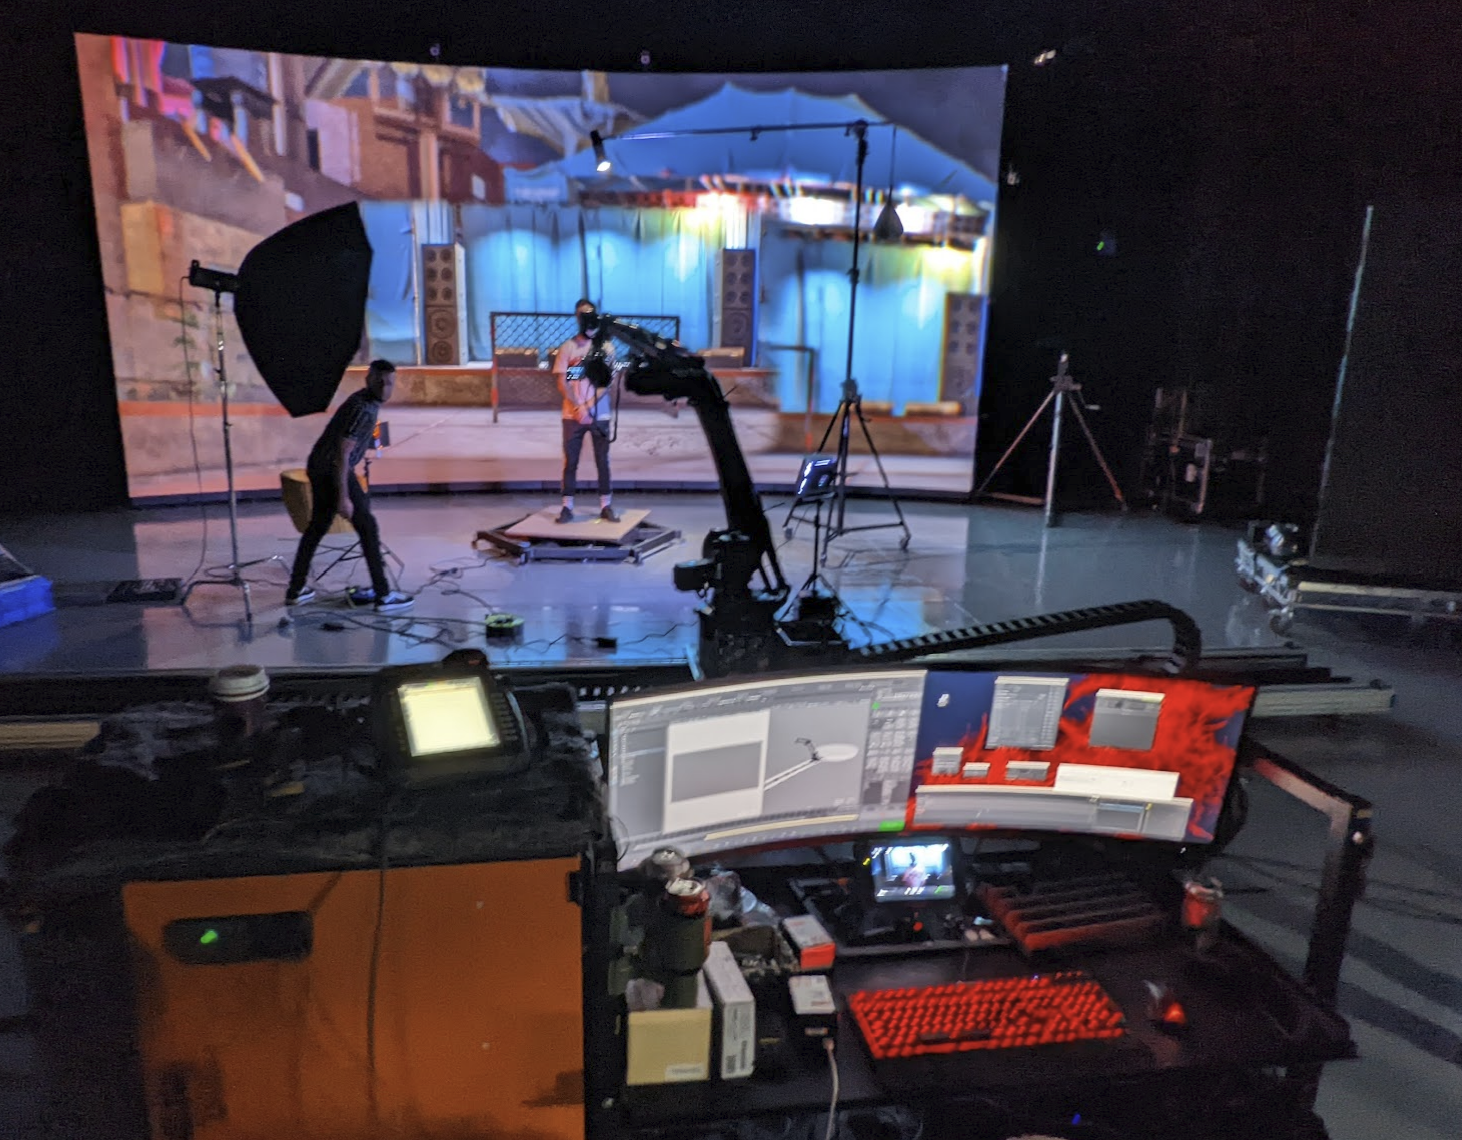
\includegraphics[width=\linewidth]{pathway}
 \caption{\href{https://www.pathwayxr.studio/}{Pathway XR virtual production}}
    \label{fig:pathway}
\end{figure}

